\documentclass{article}
\usepackage[utf8]{inputenc}
\usepackage[english]{babel}
\usepackage{indentfirst}
\usepackage{graphicx}
\usepackage{xcolor}
\usepackage{amsmath}
\usepackage{hyperref}

\newcommand{\cmd}[1]{\texttt{#1}}
\hypersetup{
	colorlinks = true,
	linkbordercolor = 1 1 1,
	urlcolor = blue,
	linkcolor = black,
	urlbordercolor = 1 1 1,
	citecolor = black
}


\title{Impressions 2D\\Rapport de la 2ème étape}
\author{}
\date{}
\addto\captionsenglish{\renewcommand*\contentsname{Sommaire}}


\pagestyle{headings}

\begin{document}

\begin{titlepage}
	\begin{center}

		% \vspace* creates some vertical white space on the page to make the title page look more pleasing.  \vspace would do much the same thing, but would not insert the white space if we were at the top of a fresh page.  As this is the start of the document we're obviously at the beginning of a page, so the asterisk is necessary to ensure we still put in two cm of white space.
		\vspace*{2cm}
		
		{\Large Services et technologies multimédia (D200006)} % \huge sets the font size.  Other options include things like \large, \Large, \small, \tiny, etc.
		
		\vspace{5cm}
		{\huge\textbf{Projet Unity, Serious Game\\Rapport de la 3ème étape:\\ }}
		
		\vspace{4cm}
		{par\\\large Dany A. DARGHOUTH \\\& Cédric PENDVILLE}
		% \vfill creates an arbitrary amount of vertical white space as necessary to fill the page
		\vfill
		
		Mai 2023
		
		% \vspace*{3cm}
		
		\end{center}
\end{titlepage}

\maketitle
\tableofcontents
\newpage

\section{Introduction}
Ce rapport accompagne le rendu de la 3ème étape d
\section{Règles du jeu}
\section{Gameplay}
\section{But du jeu}
\section{Adapatation de la difficulté}
L'adapatation de la difficulté s'eefectue de la manière suivante: Le temps que le joueur met à résoudre un niveau est mesuré, et si le temps mis est en dessous d'un certain seuil, le joueur se vera proposé un niveau présentatn une nouvelle porte logique, dans le cas contraire, le jeu lui proposera un nouveau niveau n'incluant que la/les portes qu'il connait déjà. Cette différence influear également sur le score du joueur (le meilleur score étant obtenu en résolvant tous les niveaux "assez" rapidement).\\

\begin{figure}[h]
    \centering
    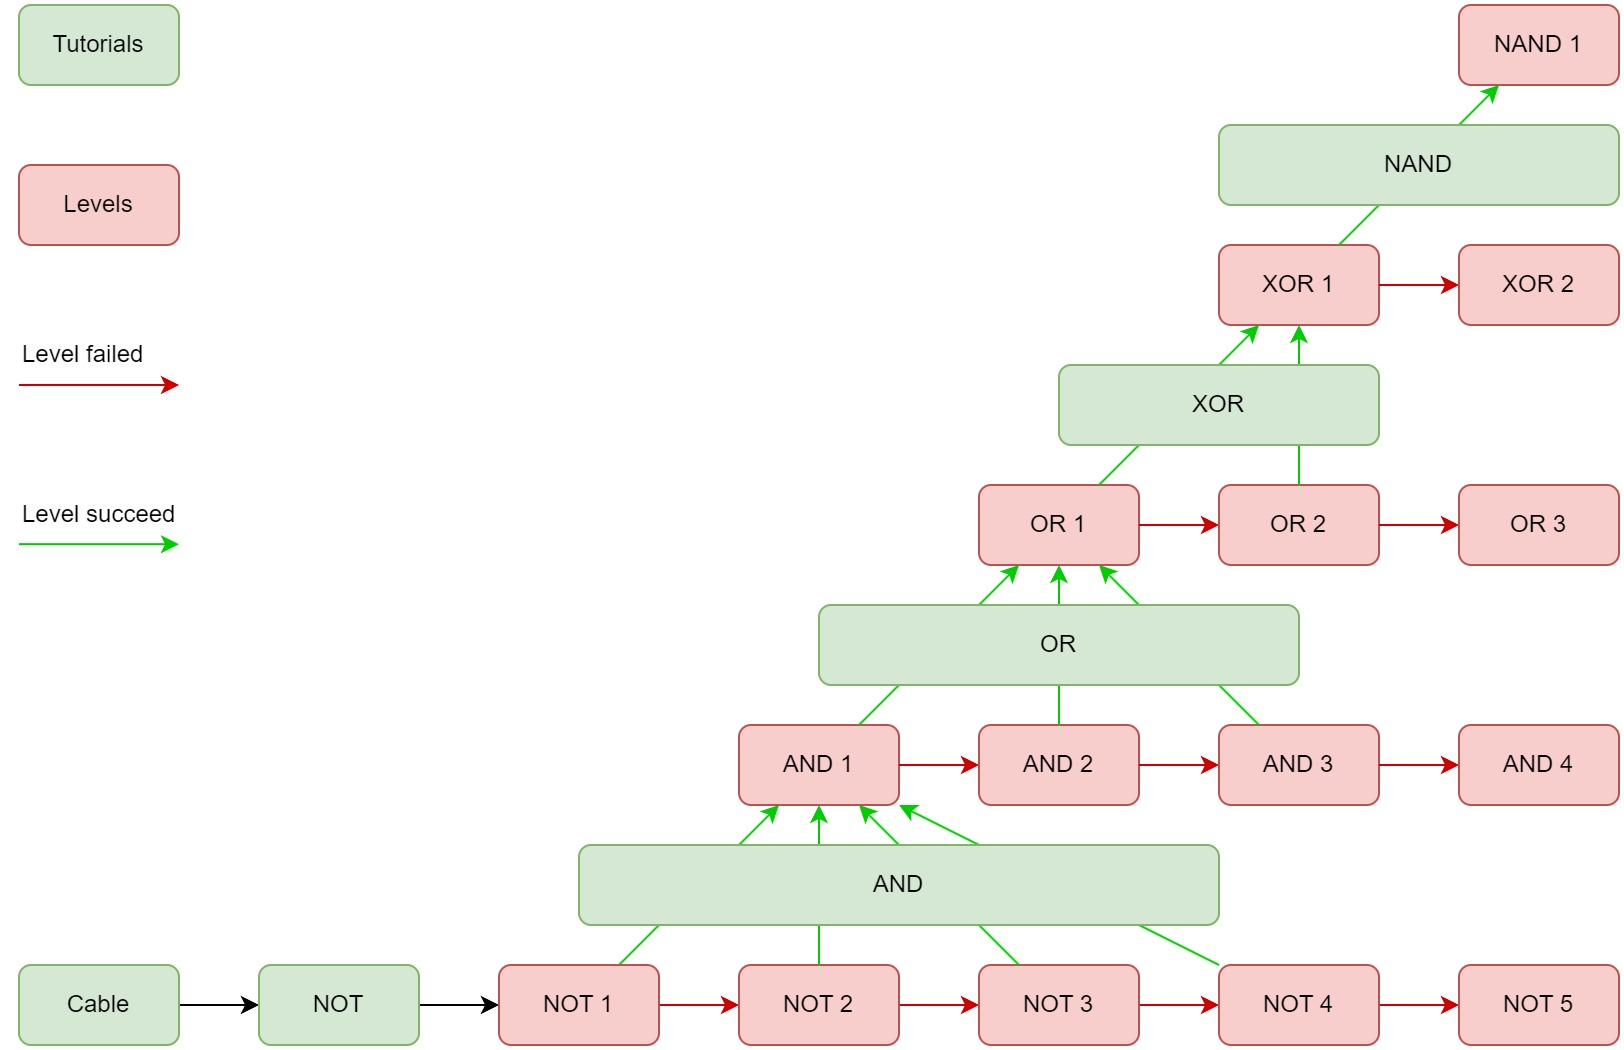
\includegraphics[width=\textwidth]{img/Levels Tree.jpg}
    \caption{Schéma de la structure des niveaux}
\end{figure}

\section{Structure du jeu}
    \subsection{Scènes}

    \subsection{GameObjects}    
    \subsection{Scripts}

\section{Evaluation du jeu}
    
\end{document}
\[\]